\PassOptionsToPackage{unicode}{hyperref}
\documentclass[aspectratio=1610, 9pt]{beamer}

% Load packages you need here
\usepackage{polyglossia}
\setmainlanguage{english}

\usepackage{csquotes}
    

\usepackage{amsmath}
\usepackage{amssymb}
\usepackage{mathtools}

\usepackage{hyperref}
\usepackage{bookmark}
\usepackage[
  locale=UK,
  separate-uncertainty=true,
  per-mode=symbol-or-fraction,
]{siunitx}
\usepackage[
  backend=biber,   % use modern biber backend
  autolang=hyphen, % load hyphenation rules for if language of bibentry is not
  % german, has to be loaded with \setotherlanguages
  % in the references.bib use langid={en} for english sources
  sorting=none,
  ]{biblatex}
  \addbibresource{references.bib}  % the bib file to use
  \DefineBibliographyStrings{english}{andothers = {{et\,al\adddot}}}  % replace u.a. with et al.
  
  
% load the theme after all packages
\usetheme[
  showtotalframes, % show total number of frames in the footline
]{tudo}

% Put settings here, like
\unimathsetup{
  math-style=ISO,
  bold-style=ISO,
  nabla=upright,
  partial=upright,
  mathrm=sym,
}
\setbeamertemplate{caption}{\raggedright\insertcaption\par}

\title{Spintronic emitters in the Terahertz Regime}
\subtitle{Applied optical spectroscopy}
\author[M.~Koch]{Max Koch}
\institute[]{TU Dortmund \\  Fakultät Physik}
%\titlegraphic{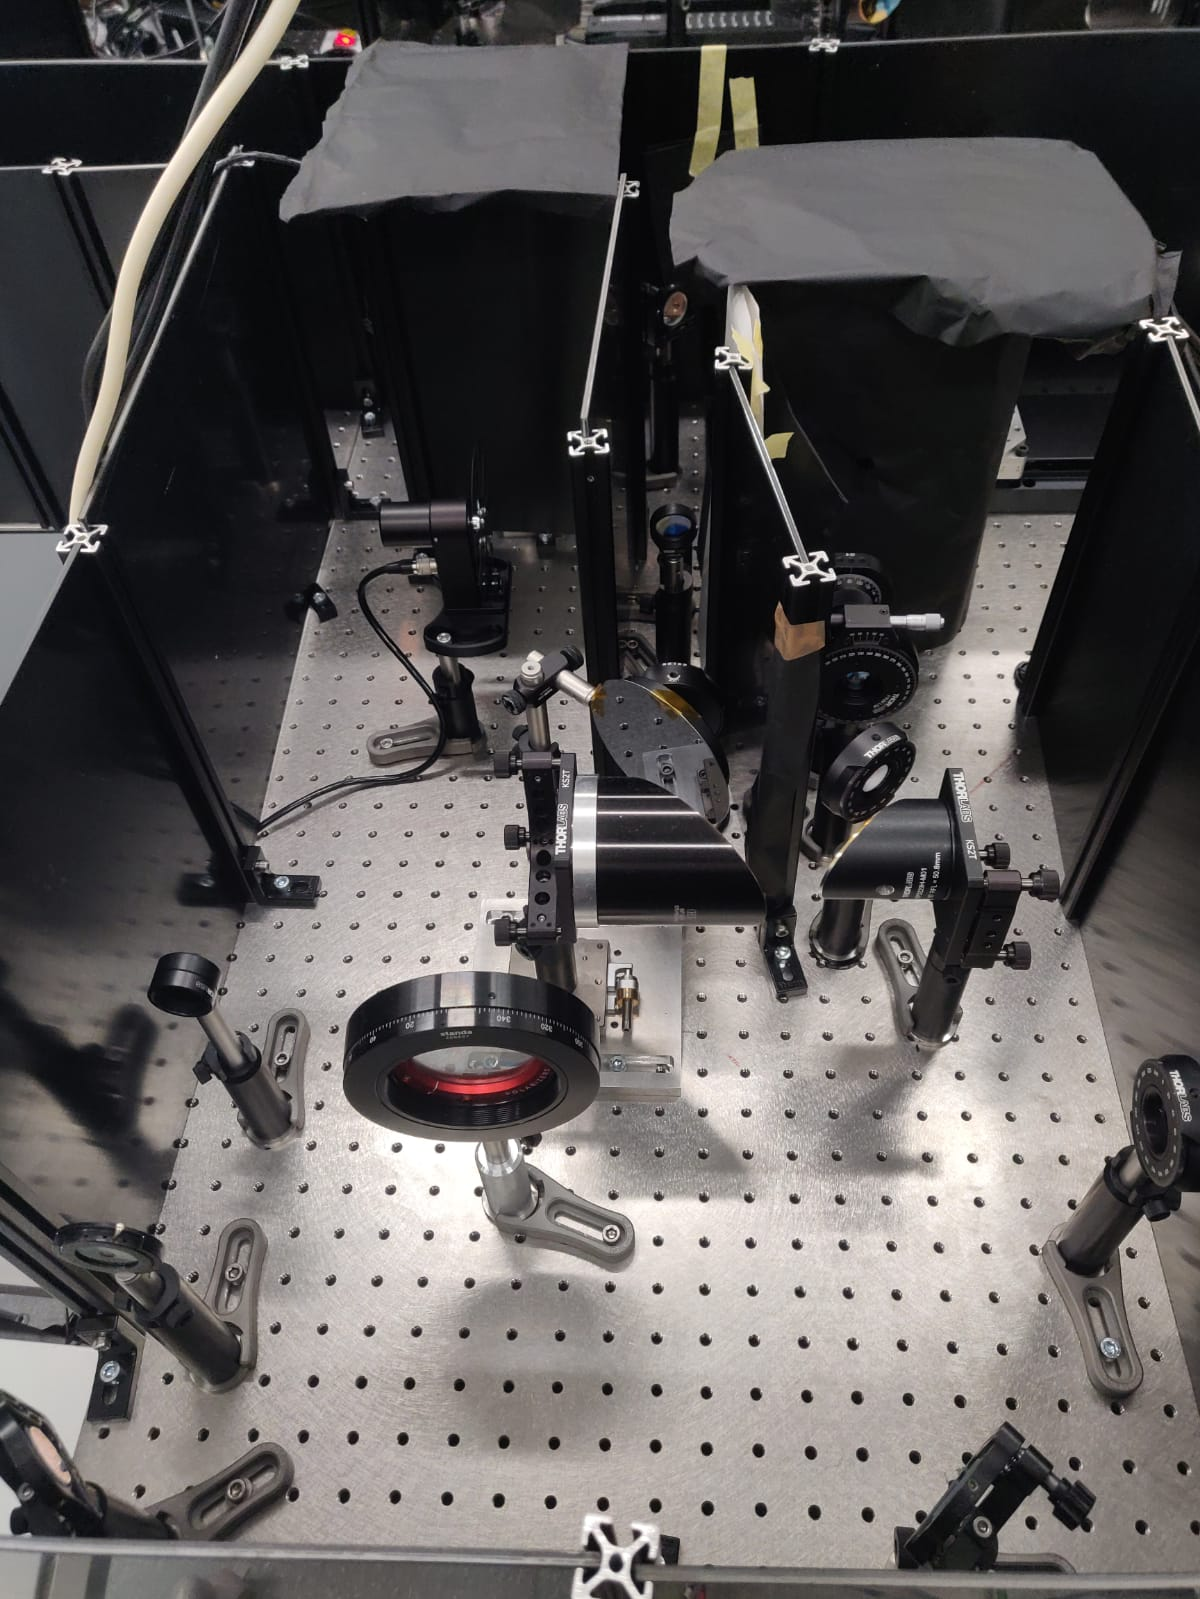
\includegraphics[width=0.3\textwidth, angle=90]{images/setup.jpeg}}


\begin{document}

\maketitle

\begin{frame}{Outline}
  \tableofcontents
\end{frame}


\section{Recap}

\begin{frame}{The THz Gap}
  \subsection{The spectrum}
  \begin{center}
    \begin{figure}
      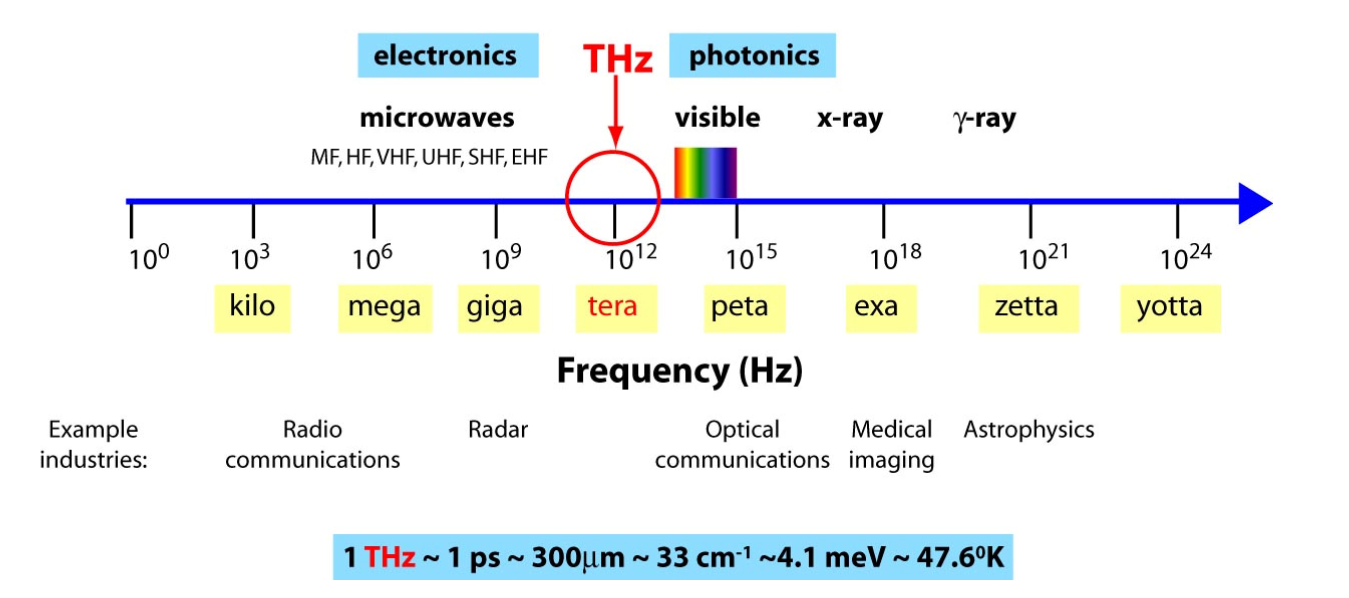
\includegraphics[width=0.7\textwidth]{images/spectrum.png}
      \caption{\textcolor{tugreen}{The electromagntic spectrum} from G. P. Williams, Rep. Prog. Phys, \textbf{69} (2005) .}
      \nocite{spectrum_pic}
    \end{figure}
  \end{center}
\end{frame}


\begin{frame}{Terahertz}
  \subsection{Applications for THz}
  \begin{center}
    \begin{minipage}[c]{0.5\linewidth}
      So why do we need terahertz radiation?
      \vspace{0.2in}
      \begin{itemize}
        \item medicine \nocite{THzgap_applications}
        \vspace{0.1in}
        \item security \nocite{thz_explosive_detec}
        \vspace{0.1in}
        \item data transmission \& saving \nocite{communication,datasaving}
        \vspace{0.1in}
        \item physics \nocite{wiki_book}
      \end{itemize}
    \end{minipage}
\end{center}
\end{frame}

\section{Introduction}
\begin{frame}{Introduction}
\begin{columns}
  \begin{column}{.3\textwidth}
    \subsection{Common emitters}
    \begin{itemize}
      \item PCA 
      \vspace{0.3in}
      \item{Non linear crystals}
    \end{itemize}
  \end{column}
  \begin{column}{.7\textwidth}
    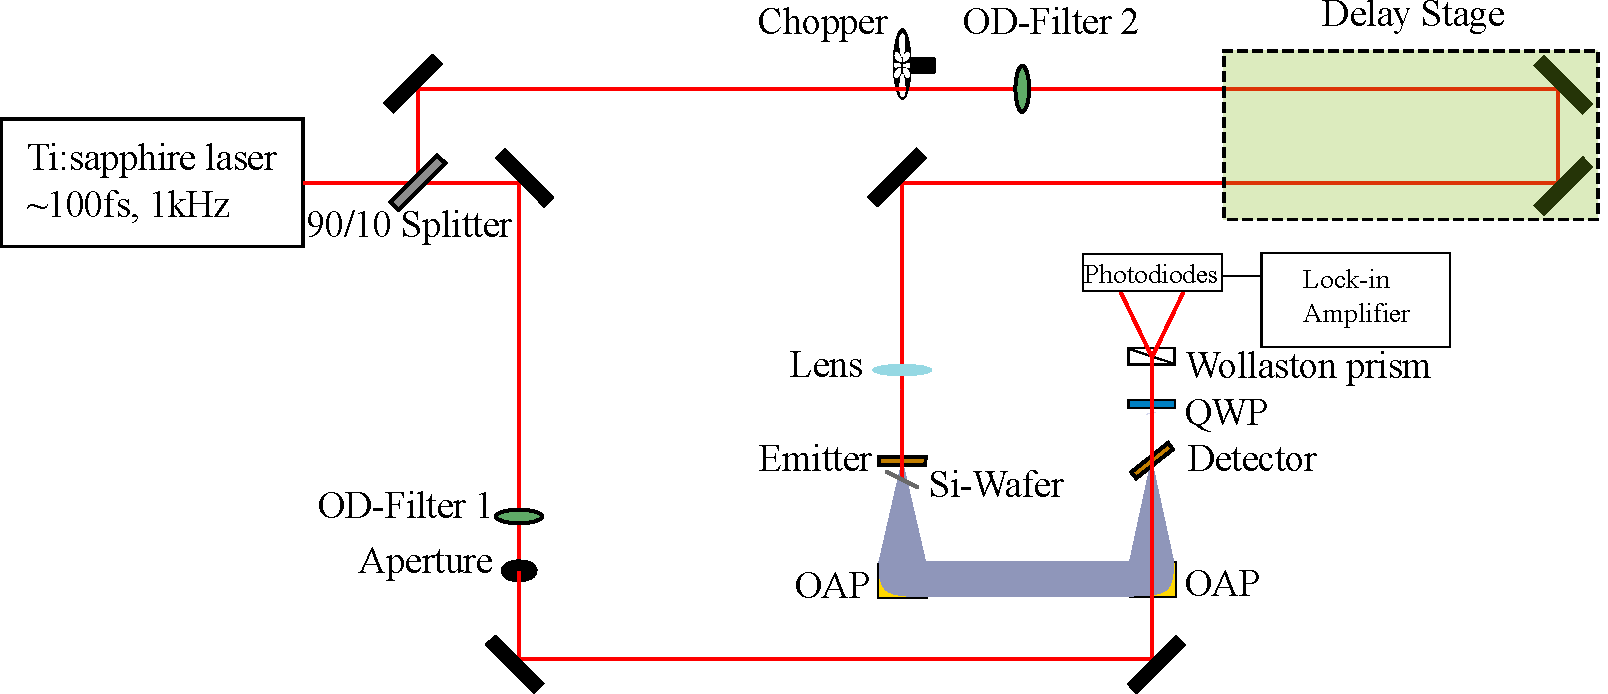
\includegraphics[width=0.7\textwidth]{images/Aufbau.pdf}
  \vspace{0.3in}
    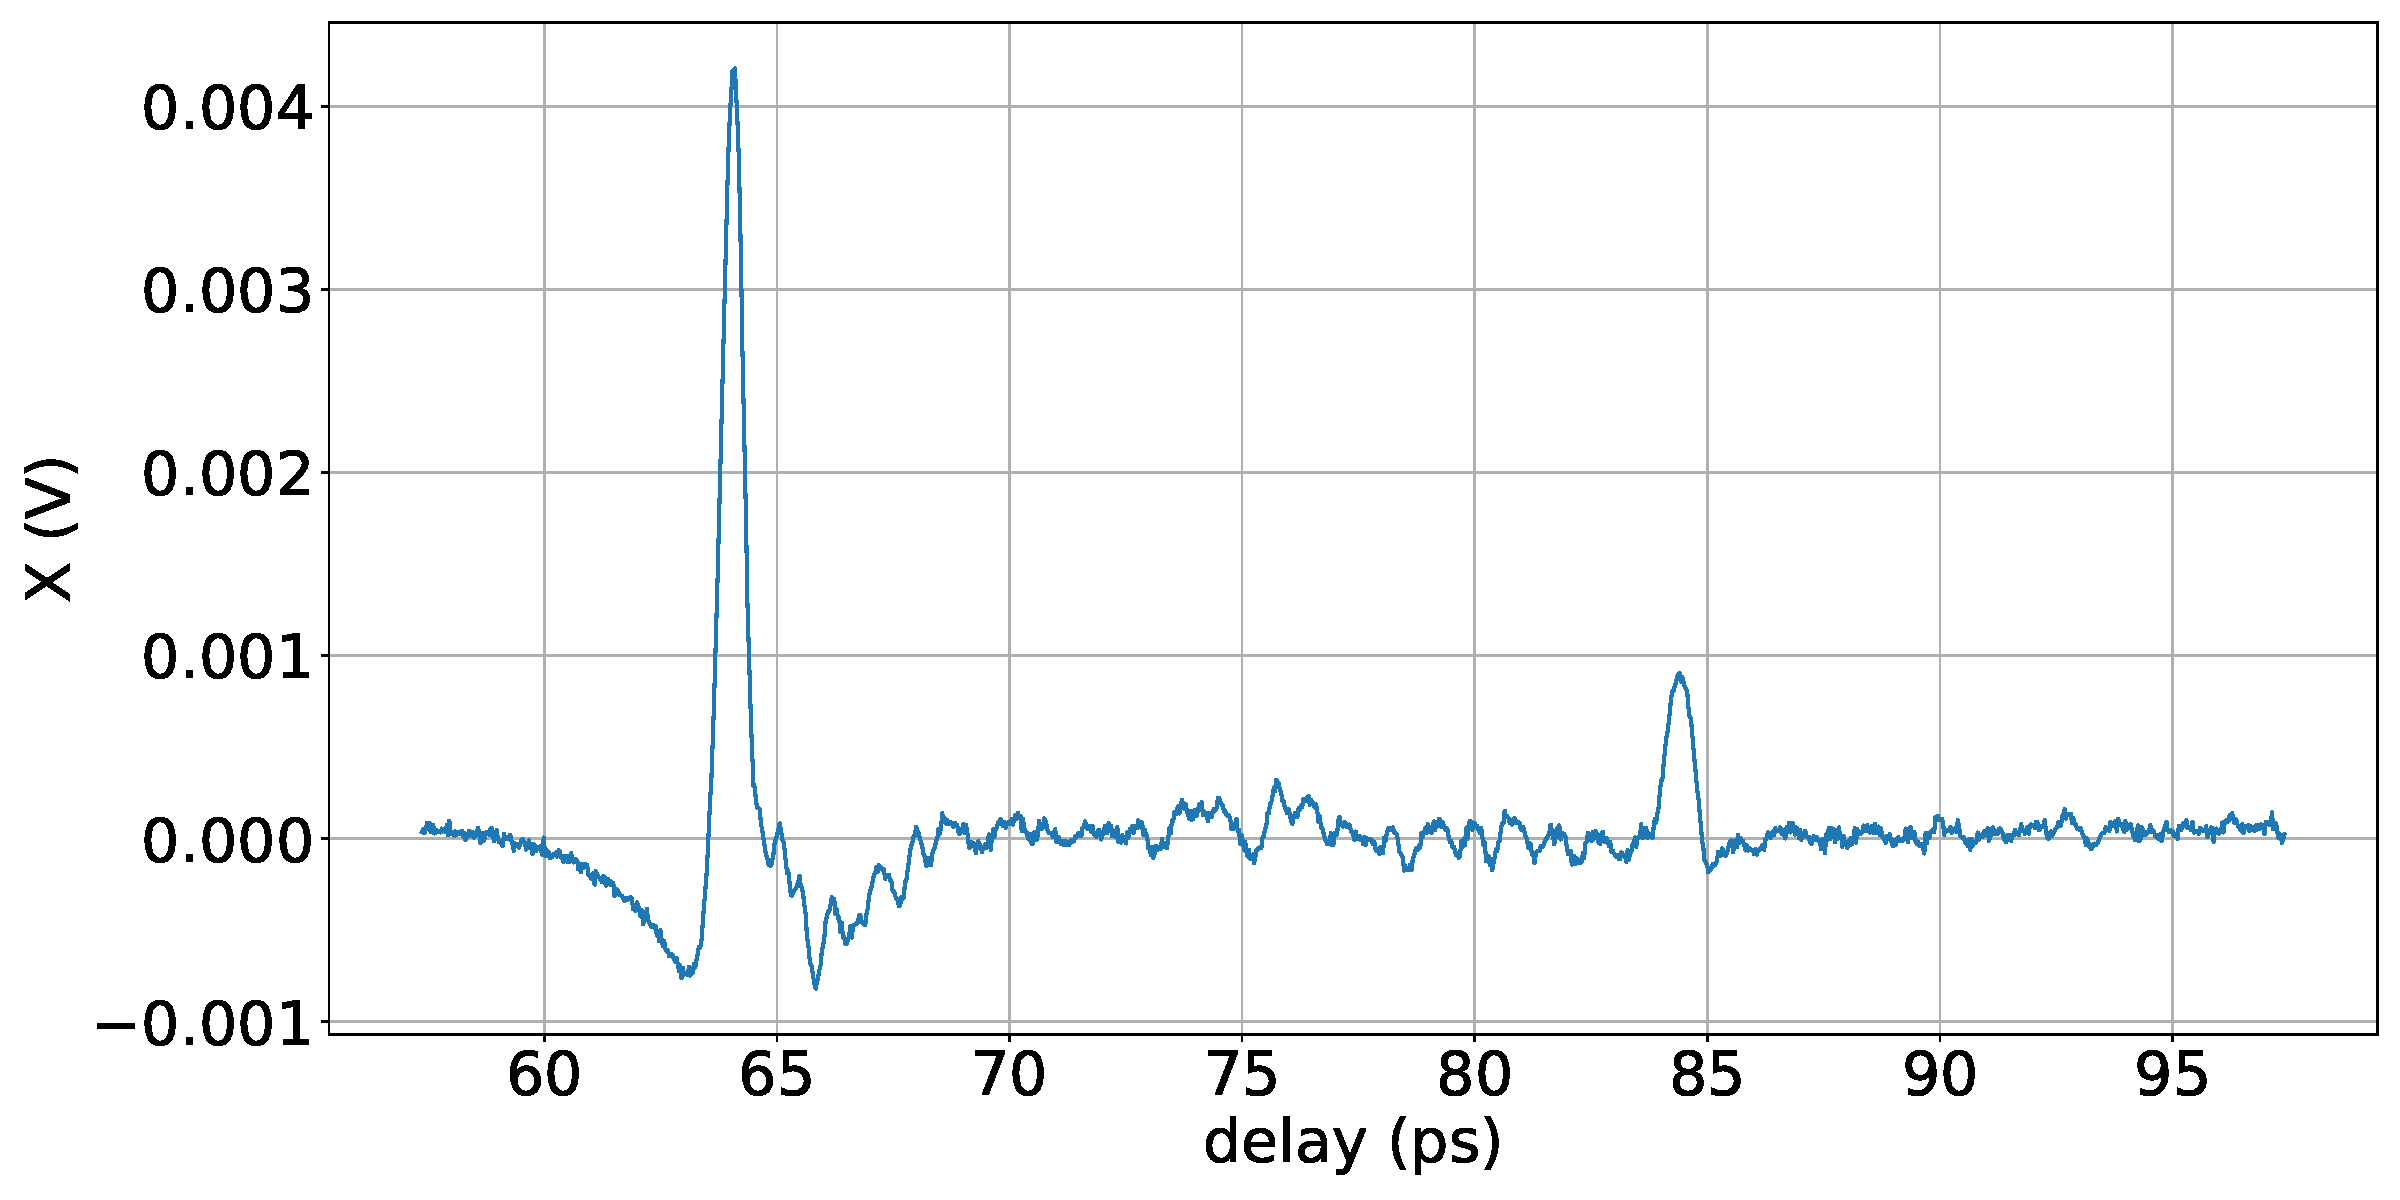
\includegraphics[width=0.7\textwidth]{images/2_11_30_20normalX.pdf}
  \end{column}
\end{columns}
\end{frame}

\begin{frame}{What are Spintronic emitters?}
  \begin{columns}
    \begin{column}{0.3\textwidth}
      \begin{itemize}
        \item Ferromagnetic Material (FM)
        \vspace{0.3in}
        \item Non Magnetic (NM)
        \vspace{0.3in}
        \item Magnetic field
      \end{itemize}
    \end{column}
    \begin{column}{.6\textwidth}
      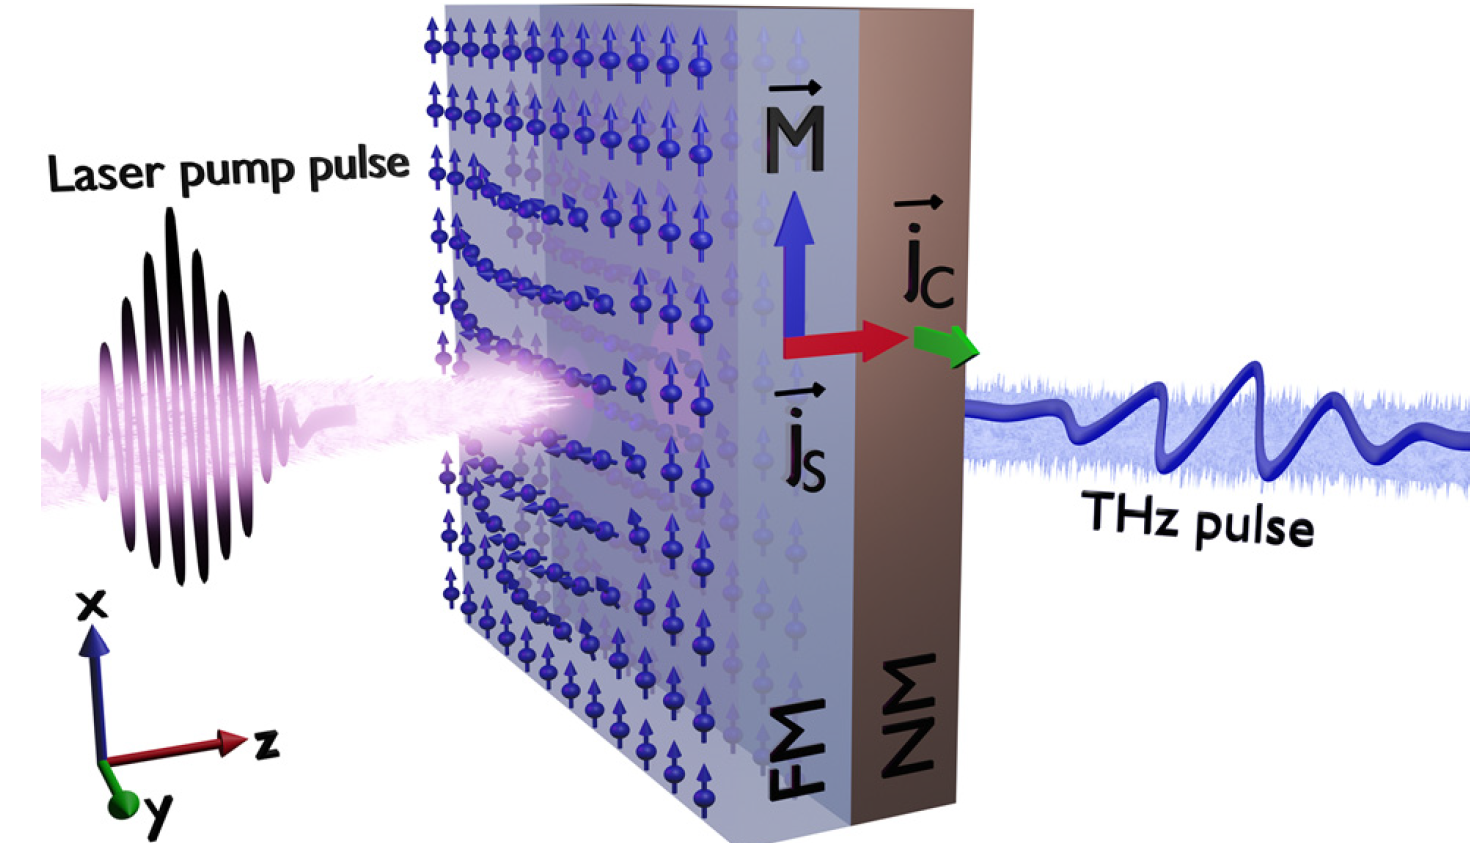
\includegraphics[width=\textwidth]{pics/emitter.png}
    \end{column}
  \end{columns}
\end{frame}

\begin{frame}{How does it work?}
  \begin{center}
  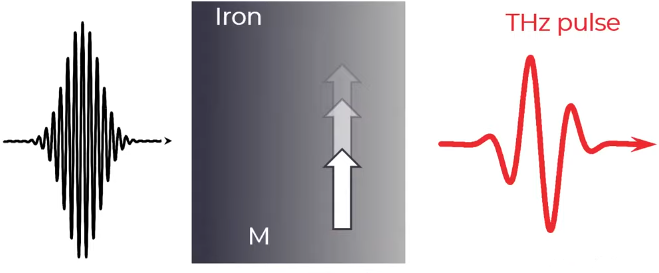
\includegraphics[width=0.6\textwidth]{pics/quenching.png}
  \end{center}
  \begin{equation}
    E_\text{DM} \propto \dot{M}(t)
  \end{equation}
\end{frame}

\begin{frame}{Stronger if we attach NM}
  \begin{columns}
    \begin{column}{0.6\textwidth}
    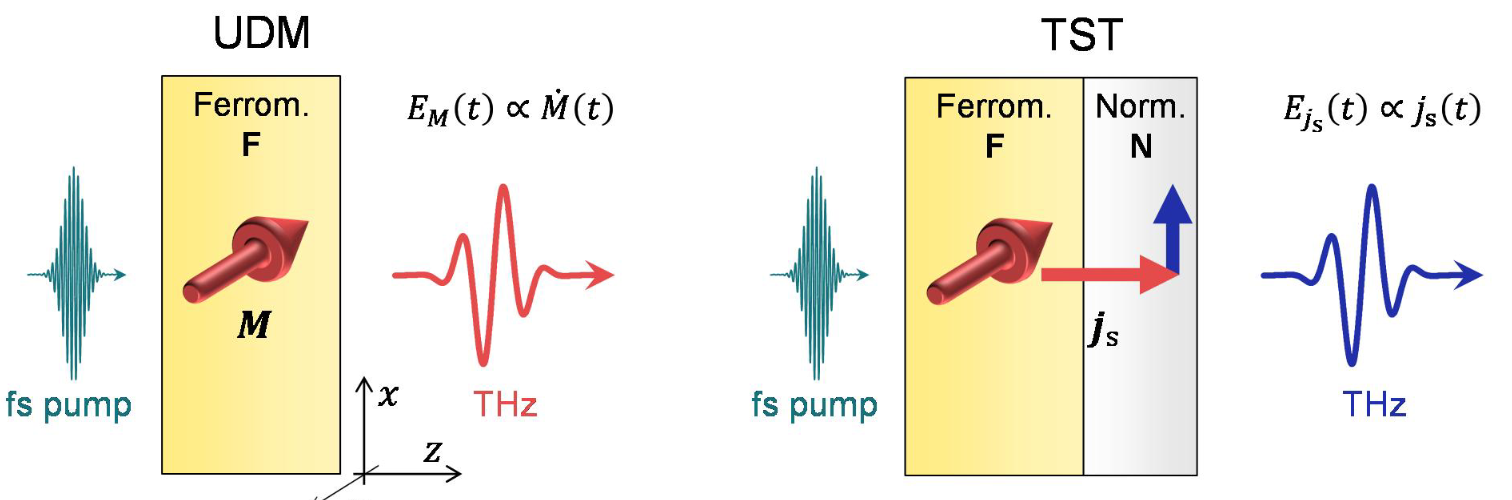
\includegraphics[width=\textwidth]{pics/FMNM.png}
    \nocite{arxiv}
    \end{column}
    \begin{column}{0.4\textwidth}
      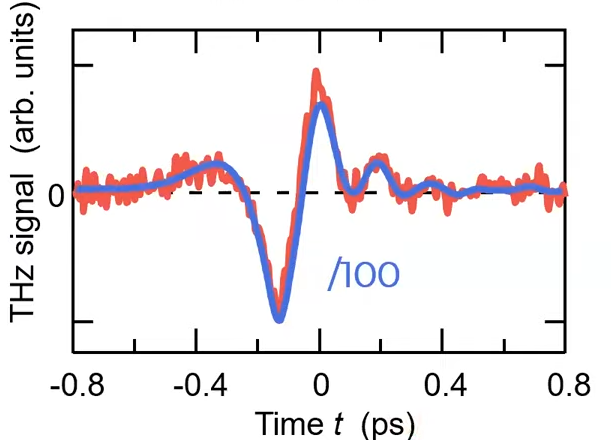
\includegraphics[width=\textwidth]{pics/FM-vsdouble.png}
    \end{column}
  \end{columns}
\end{frame}

\section{Inverse Spin Hall effect}
\begin{frame}{Where does the current come frome?}
\begin{center}
Inverse Spin Hall effect!
\end{center}
\begin{columns}
  \begin{column}{0.5\textwidth}
  Spin Hall effect
  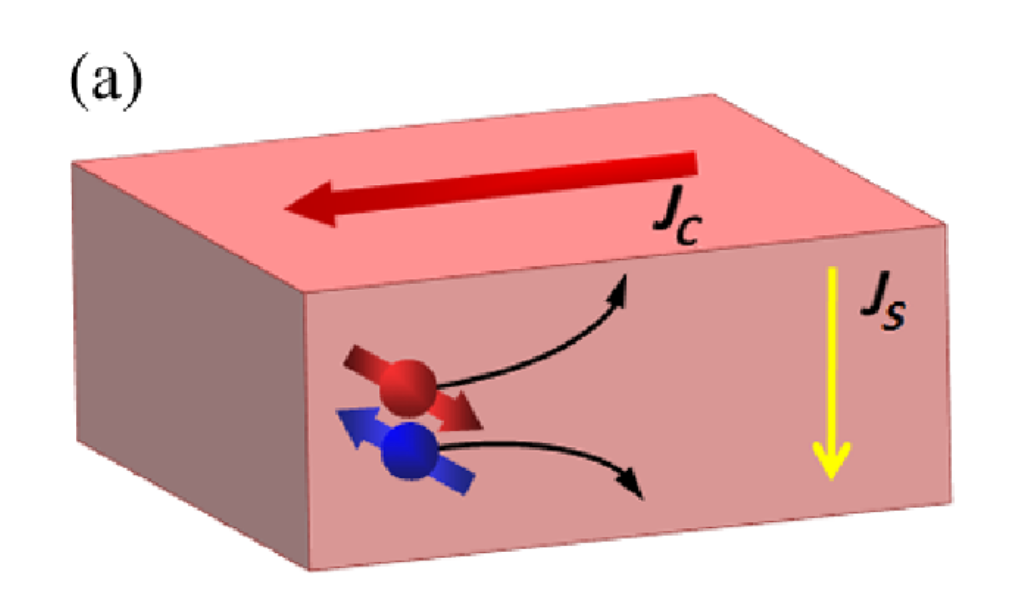
\includegraphics[width=\textwidth]{pics/Spin_Hall.png}
  \end{column}
  \begin{column}{0.5\textwidth}
    Inverse Spin Hall effect
    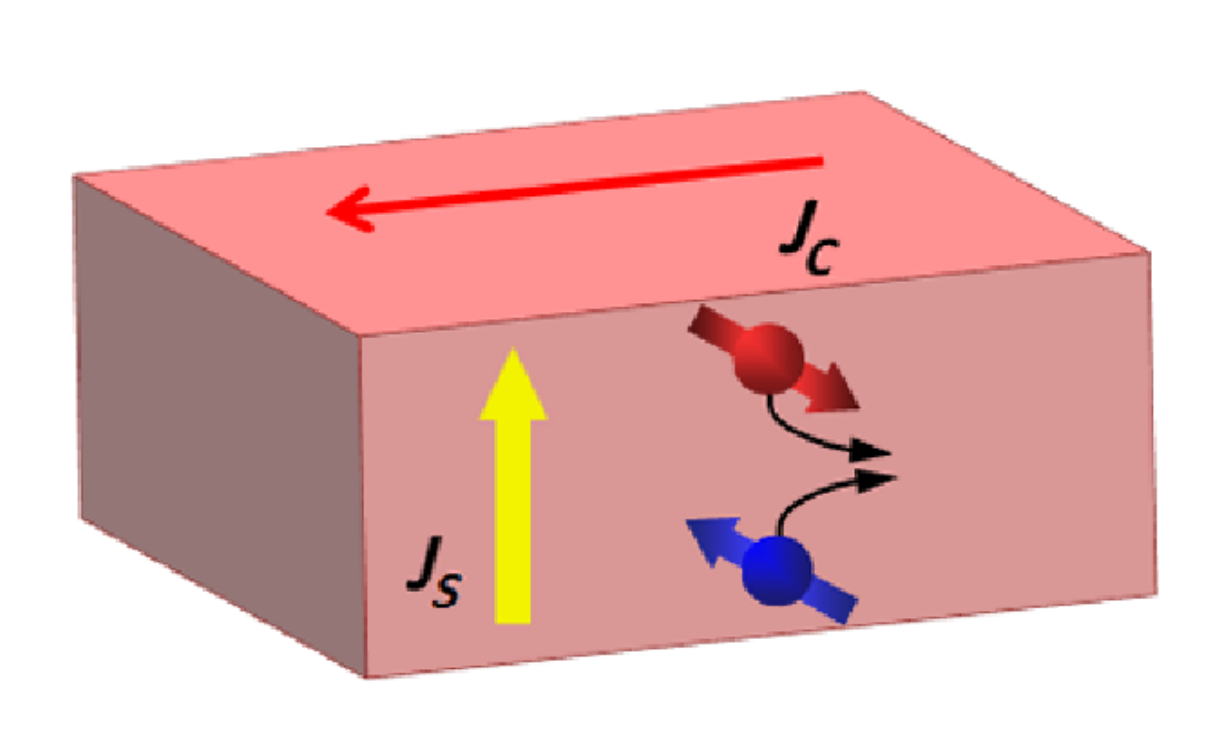
\includegraphics[width=\textwidth]{pics/inv_spin_hall.png}
  \end{column}
\end{columns}
\end{frame}

\begin{frame}{2 Layers are not the end}
  \begin{columns}
    \begin{column}{0.5\textwidth}
      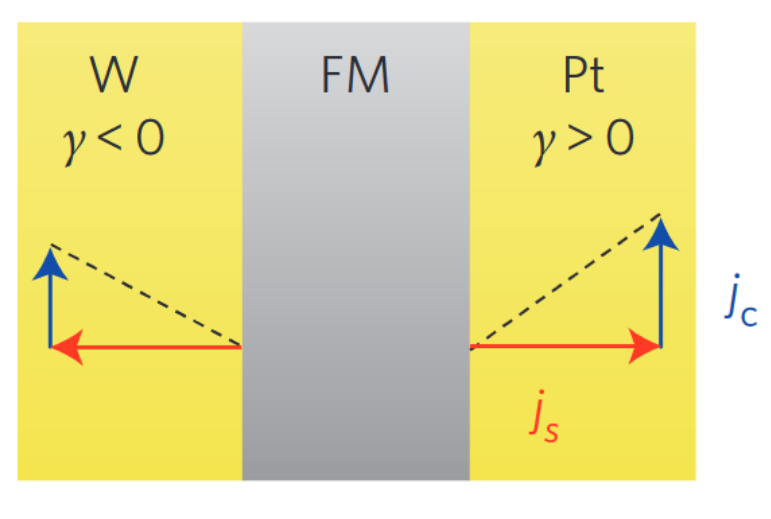
\includegraphics[width=.8\textwidth]{pics/trilayer.png}
    \end{column}
    \begin{column}{.5\textwidth}
    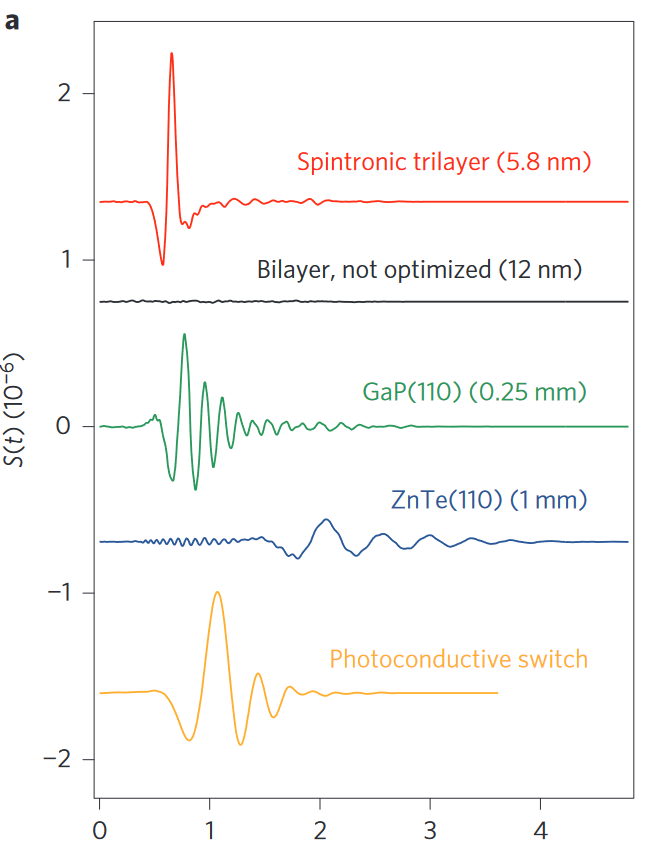
\includegraphics[width=.6\textwidth]{pics/vergleich.png}
    \end{column}
  \end{columns}
\end{frame}

\section{Advantages}
\begin{frame}{Polarization}
  \begin{center}
    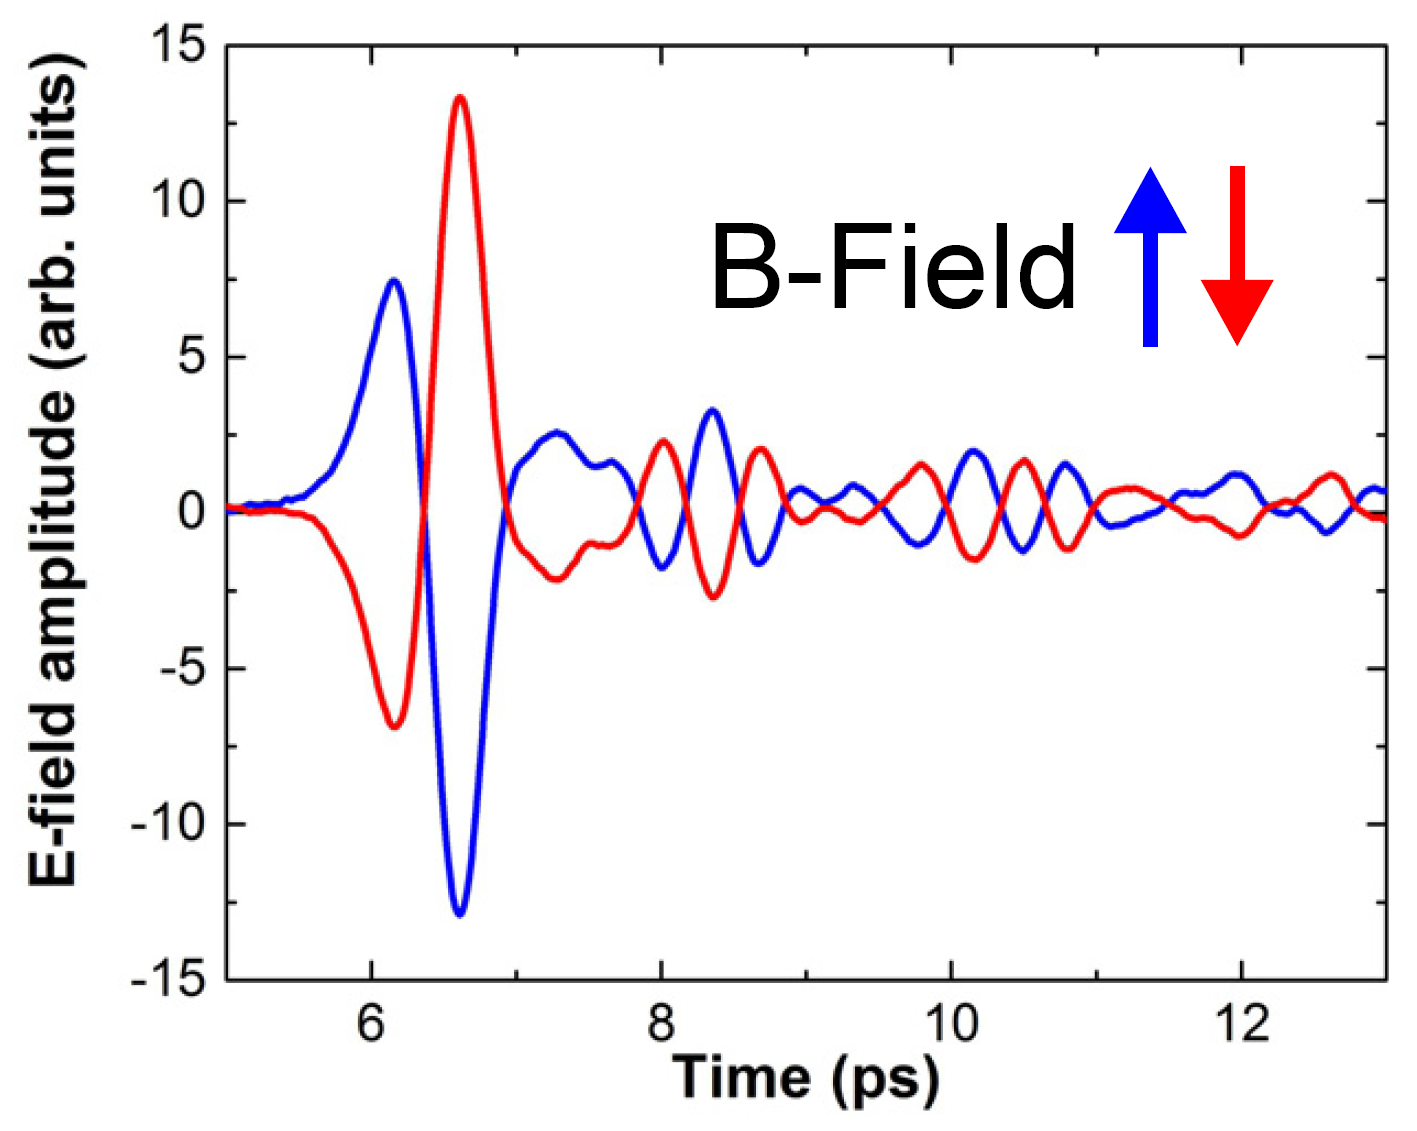
\includegraphics[width=0.4\textwidth]{pics/Bfeld.png}
  \end{center}
\end{frame}

\begin{frame}{Broadband}
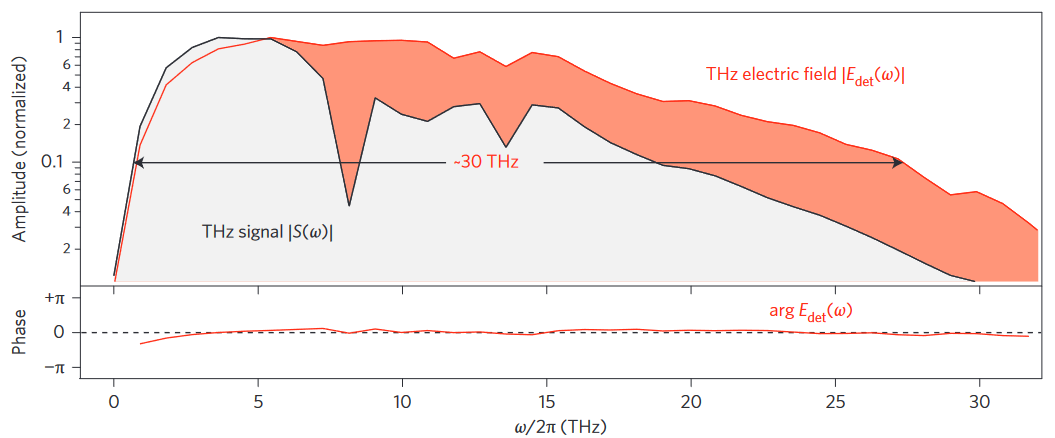
\includegraphics[width=\textwidth]{pics/broadband.png}
\end{frame}



\section*{Thank you}
\begin{frame}{}
  \begin{center}
  \textbf{\textcolor{tugreen}{Thank you all for your attention!}}
  \end{center}
\end{frame}

\section{References }
\printbibliography

\end{document}

